\documentclass[final]{article}

% --- Paper size: 36in x 24in landscape ---
\usepackage[paperwidth=36in, paperheight=24in,
            margin=0in]{geometry}

\usepackage[T1]{fontenc}
\usepackage[utf8]{inputenc}
\usepackage{helvet}
\renewcommand{\familydefault}{\sfdefault}

\usepackage{graphicx}
\usepackage{xcolor}
\usepackage{booktabs}
\usepackage{array}
\usepackage{colortbl}
\usepackage{enumitem}
\usepackage{tikz}
\usepackage{amsmath}
\usepackage[most]{tcolorbox}
\usepackage{ragged2e}
\usepackage[absolute,overlay]{textpos}

\pagestyle{empty}
\pagenumbering{gobble}
\setlength{\parindent}{0pt}
\setlength{\parskip}{0.25em}
\setlength{\tabcolsep}{6pt}

% textpos uses inches throughout
\setlength{\TPHorizModule}{1in}
\setlength{\TPVertModule}{1in}
\TPGrid{36}{24}

% --- Palette ---
\definecolor{cornellred}{RGB}{179,27,27}
\definecolor{darkink}{RGB}{33,37,43}
\definecolor{bodyink}{RGB}{52,58,64}
\definecolor{subtle}{RGB}{236,238,241}
\definecolor{accent}{RGB}{20,96,158}
\definecolor{highlight}{RGB}{255,243,205}

\color{bodyink}

% --- Font-size helpers (poster-scale) ---
\newcommand{\titlefs}{\fontsize{68}{80}\selectfont}
\newcommand{\authorfs}{\fontsize{28}{34}\selectfont}
\newcommand{\colheadfs}{\fontsize{40}{48}\selectfont}
\newcommand{\subheadfs}{\fontsize{26}{32}\selectfont}
\newcommand{\bodyfs}{\fontsize{21}{26}\selectfont}
\newcommand{\tabfs}{\fontsize{19}{24}\selectfont}
\newcommand{\tinyfs}{\fontsize{17}{21}\selectfont}

\newcommand{\colhead}[1]{{\colheadfs\bfseries\color{cornellred}#1}\\[-0.2em]\textcolor{cornellred}{\rule{\linewidth}{2.2pt}}\vspace{0.10in}}
\newcommand{\subhead}[1]{\vspace{0.12in}{\subheadfs\bfseries\color{darkink}#1}\vspace{0.04in}\\}

\setlist[itemize]{leftmargin=1.1em, topsep=0.05em, itemsep=0.18em, parsep=0.05em,
  label=\textcolor{cornellred}{\textbullet}}

\renewcommand{\arraystretch}{1.15}

\begin{document}
\null % a page to attach textblocks to

% ============================================================
% TITLE BAR (full width, y=0.7 to y=2.3)
% ============================================================
\begin{textblock}{34.5}(0.75, 0.45)
\bodyfs\RaggedRight
\begin{center}
{\titlefs\bfseries\color{darkink}Detecting Inferior Myocardial Infarction\\from a Single ECG Lead}\\[0.15em]
{\authorfs\color{bodyink}Gabriel Butler \;\textperiodcentered\; Cornell University \;\textperiodcentered\; CS 5782, Spring 2026}
\end{center}
\vspace{0.12in}
\textcolor{cornellred}{\rule{\linewidth}{4pt}}
\end{textblock}

% ============================================================
% COLUMN 1 (x=0.75, y=3.1, w=10.9)
% ============================================================
\begin{textblock}{10.9}(0.75, 3.7)
\bodyfs\RaggedRight
\colhead{1. Background \& Motivation}

\subhead{What is an ECG?}
\begin{itemize}
  \item Records the heart's electrical activity from electrodes on the body
  \item Used to screen for arrhythmias, ischemia, and \textbf{myocardial infarction (MI)} --- ``heart attack''
\end{itemize}

\subhead{What is a ``lead''?}
\begin{itemize}
  \item A specific viewing angle of the heart, defined by a pair of electrodes. A clinical ECG uses \textbf{12 leads}, each looking at the heart from a different direction
  \item \textbf{Lead I} runs horizontally across the chest (left arm $-$ right arm) and is the only lead captured by most cheap, single-lead devices (Apple Watch, KardiaMobile, handheld rural-clinic tools)
  \item \textbf{Inferior MI} damages the bottom wall of the heart. Its signal projects onto the \emph{inferior} leads (II, III, aVF), nearly orthogonal to Lead I --- clinicians consider Lead I \emph{blind} to inferior MI
\end{itemize}

\subhead{What Obermeyer et al.\ (2026) did}
A two-stage training recipe for MI screening on cheap hardware:
\begin{itemize}
  \item \textbf{Pretrain on Sweden:} a large EHR-derived dataset of 12-lead ECGs from a Swedish hospital system. Lead I was extracted and processed to approximate a handheld device's waveform; the model (an 18-layer 1D ResNet) predicts an \emph{ICD-coded prior MI} diagnosis
  \item \textbf{Fine-tune on rural Tamil Nadu, India:} the authors collected a new dataset of 5{,}301 adults aged $\geq$40 via health camps across five districts, using a \textbf{\$60 AliveCor KardiaMobile} single-lead ECG. The fine-tuning target is \emph{regional wall motion abnormality} on echocardiography --- a proxy for prior MI
  \item \textbf{Headline result:} AUC \textbf{0.77} on a 60\% held-out slice of the Tamil Nadu cohort; top 2.5\% of scores show $\sim$6$\times$ enrichment over the $\sim$1.5\% base rate; screening is cost-effective at \$1{,}999 per life-year saved
\end{itemize}

\subhead{Our replication \& extension}
\begin{itemize}
  \item We mirror the \emph{train-in-developed, deploy-in-developing} structure with public data: \textbf{Germany (PTB-XL) $\rightarrow$ China (Ningbo+Shaoxing)}
  \item Original paper never addresses \emph{on-device inference}. We add an architecture sweep, INT8 quantization, and real-phone latency profiling via Qualcomm AI Hub
\end{itemize}
\end{textblock}

% ============================================================
% COLUMN 2 (x=12.55, y=3.1, w=10.9)
% ============================================================
\begin{textblock}{10.9}(12.55, 3.7)
\bodyfs\RaggedRight
\colhead{2. Methods}

\subhead{Architectures}

\begin{center}
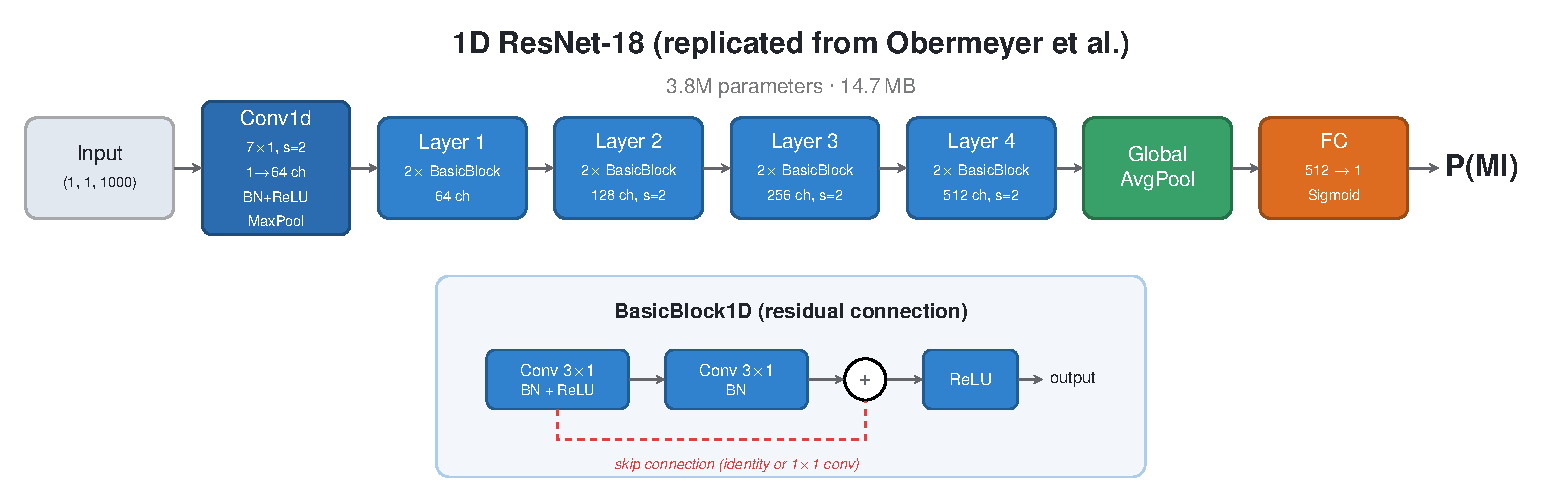
\includegraphics[width=\linewidth]{resnet18_diagram.pdf}\\[0.12in]
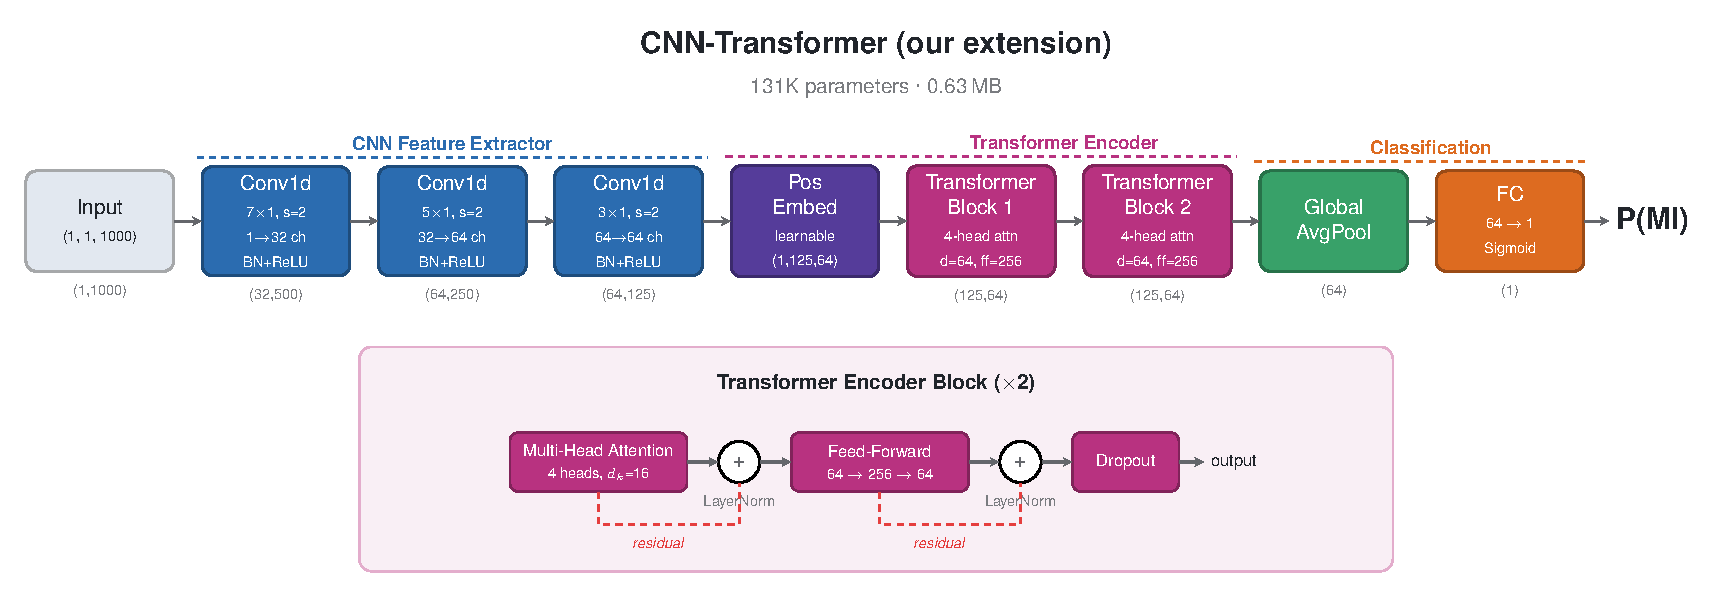
\includegraphics[width=\linewidth]{cnn_transformer_diagram.pdf}
\end{center}

\subhead{Architecture sweep (40/60 split)}

\begin{center}
\tabfs
\begin{tabular}{@{}l r r r@{}}
\toprule
\textbf{Architecture} & \textbf{Params} & \textbf{Size} & \textbf{AUC} \\
\midrule
Mamba-ECG                                  & 104K & 0.42\,MB & 0.863 \\
\rowcolor{highlight}\textbf{ResNet-18 (orig.)}                 & 3.8M & 14.7\,MB & 0.852 \\
\rowcolor{highlight}\textbf{CNN-Transformer (ours)}            & 131K & 0.52\,MB & 0.851 \\
ResNet-34                                   & 7.2M & 27.7\,MB & 0.848 \\
ResNet-18 + CBAM                            & 3.9M & 15.1\,MB & 0.844 \\
ResNet-50                                   & 16M  & 61.2\,MB & 0.805 \\
Tiny Transformer                            & 4.4K & 0.02\,MB & 0.729 \\
\bottomrule
\end{tabular}
\end{center}

\subhead{Training}
\textbf{Pretrain} PTB-XL (Lead I) $\rightarrow$ \textbf{zero-shot} eval on Chinese set $\rightarrow$ \textbf{fine-tune} Ningbo+Shaoxing $\rightarrow$ \textbf{test} on held-out Chinese split. Focal loss ($\alpha{=}0.25, \gamma{=}2.0$), Adam, 5-epoch warmup + cosine; augment: noise, amplitude scale, time shift.

\subhead{Data splits}
\begin{center}
\tabfs
\begin{tabular}{@{}l l l l@{}}
\toprule
\textbf{Dataset (split)}                     & \textbf{Train} & \textbf{Val} & \textbf{Test} \\
\midrule
PTB-XL (patient, folds 1-8/9/10)             & 17,418 / 25\% MI & 2,183 & 2,198 \\
Ningbo+Shaoxing (40/20/40, MI-strat.)        & 18,060 / 49 MI   & 9,030 / 25 MI & 18,062 / 49 MI \\
\bottomrule
\end{tabular}
\end{center}
{\tinyfs Only \textbf{49 MI cases} in fine-tune train --- data is the bottleneck, not architecture.}
\end{textblock}

% ============================================================
% COLUMN 3 (x=24.35, y=3.1, w=10.9)
% ============================================================
\begin{textblock}{10.9}(24.35, 3.7)
\bodyfs\RaggedRight
\colhead{3. Results \& Deployment}

\subhead{Headline (CNN-Transformer, final)}
\begin{center}
\begin{tcolorbox}[colback=subtle, colframe=cornellred, boxrule=1.2pt, arc=3mm, left=8pt, right=8pt, top=5pt, bottom=5pt, width=0.96\linewidth]
\bodyfs
\begin{tabular}{@{}l l@{}}
Val AUC (Chinese val)                & \textbf{0.86} \\
Test AUC (held-out Chinese)          & \textbf{0.81} \\
Zero-shot AUC (no Chinese fine-tune) & 0.81 \\
Model size (FP32)                    & \textbf{0.63\,MB} \\
\end{tabular}
\end{tcolorbox}
\end{center}

\subhead{Risk stratification}
\begin{itemize}
  \item Model outputs risk \emph{scores}, not binary diagnoses (Obermeyer framing)
  \item \textbf{Top 2.5\% of scores: 7.3$\times$ enrichment} over dataset base rate --- useful for triage, not standalone diagnosis
\end{itemize}

\subhead{What is quantization?}
\begin{itemize}
  \item Neural nets normally store weights in 32-bit float (FP32). \textbf{Quantization} replaces them with 8-bit integers (INT8)
  \item Yields $\sim$4$\times$ smaller models, lower memory bandwidth, often faster mobile-NPU inference
  \item We use \textbf{post-training static quantization} (ONNX Runtime, QDQ format), calibrating activation ranges on a small Chinese-ECG sample
\end{itemize}

\subhead{On-device (Qualcomm AI Hub)}
\begin{center}
\tabfs
\begin{tabular}{@{}l c c c c@{}}
\toprule
\textbf{Precision} & \textbf{AUC} & \textbf{Size} & \textbf{S24} & \textbf{Redmi 10} \\
\midrule
FP32 & 0.855 & 0.63\,MB & \textbf{152\,$\mu$s} & \textbf{1,960\,$\mu$s} \\
INT8 & 0.855 & 0.19\,MB & \textcolor{cornellred}{failed} & 4,158\,$\mu$s \\
\bottomrule
\end{tabular}
\end{center}
\vspace{0.04in}
\begin{itemize}
  \item Targets: Samsung Galaxy S24 (flagship) \& Xiaomi Redmi Note 10 5G ($\sim$\$100 LMIC-tier phone)
  \item INT8 shrinks size 3.3$\times$ with \textbf{99.9\% AUC retention}; on this model size, FP32 is already faster, and INT8 QNN compilation fails on S24
  \item \textbf{Deployment recommendation: ship FP32}
\end{itemize}

\subhead{Comparison with Obermeyer et al.}
\begin{center}
\tabfs
\begin{tabular}{@{}l l l@{}}
\toprule
                   & \textbf{Obermeyer 2026}       & \textbf{Ours} \\
\midrule
Pretrain / deploy pops. & Sweden $\rightarrow$ Tamil Nadu, India & Germany $\rightarrow$ Ningbo+Shaoxing, China \\
Model                   & 1D ResNet-18                          & CNN-Transformer (131K) \\
Lead(s)                 & Lead I only                           & Lead I only \\
Target                  & RWMA on echo (prior-MI proxy)         & MI label from ECG database \\
Headline AUC            & 0.77                                  & 0.81 (held-out test) \\
Top-2.5\% enrichment    & $\sim$6$\times$                       & 7.3$\times$ \\
On-device?              & not addressed                         & \textbf{1.96\,ms / \$100 phone} \\
\bottomrule
\end{tabular}
\end{center}
{\tinyfs Different targets, different populations, similar single-lead regime. Our higher AUC likely reflects the cleaner ECG-database MI labels vs.\ Obermeyer's echo-based RWMA proxy.}
\end{textblock}

% ============================================================
% BOTTOM STRIP (y=21.2)
% ============================================================
\begin{textblock}{34.5}(0.75, 21.45)
\textcolor{cornellred}{\rule{\linewidth}{3pt}}
\end{textblock}

\begin{textblock}{21}(0.75, 21.7)
\bodyfs\RaggedRight
{\subheadfs\bfseries\color{cornellred}Takeaways}\\[0.08in]
\begin{itemize}
  \item Single-lead inferior-MI detection \textbf{transfers across populations} (Europe\,$\rightarrow$\,Asia, mirroring Sweden\,$\rightarrow$\,India)
  \item A \textbf{CNN-Transformer (131K params)} matches ResNet-18 AUC at \textbf{1/29th} the size, with on-device parity
  \item \textbf{$<$\,2\,ms on a \$100 phone} --- viable for real-world LMIC screening with $\sim$\$60 single-lead hardware
  \item \textbf{INT8 not worth it at this scale}: model is already small enough that FP32 is faster and avoids mobile toolchain issues
\end{itemize}
\end{textblock}

\begin{textblock}{13}(22.25, 21.7)
\tinyfs\RaggedRight
{\subheadfs\bfseries\color{cornellred}References \& Acknowledgements}\\[0.08in]
\begin{itemize}
  \item Obermeyer et al.\ (2026), \emph{NBER WP 34690}
  \item Wagner et al., \emph{PTB-XL} (PhysioNet)
  \item Zheng et al.\ (2020), \emph{Ningbo + Shaoxing 12-lead ECG DB} (PhysioNet)
  \item Qualcomm AI Hub (on-device profiling)
  \item Completed for CS 5782, Cornell (Spring 2026)
\end{itemize}
\end{textblock}

\end{document}
